%Template Assets:
%TeX: http://www.jucs.org/ujs/jucs/info/submissions/jucs_sample_paper_latex.tex
%Style: http://www.jucs.org/ujs/jucs/info/submissions/jucs2e.sty

\documentclass[10pt,a4paper]{article}

\usepackage{jucs2e}
\usepackage{graphicx}
\usepackage{url}
\usepackage{ulem}
\usepackage{mathtools}
\usepackage{verbatim}
\usepackage{xcolor}
\usepackage[utf8]{inputenc}

% https://tex.stackexchange.com/a/2774/54244
\usepackage{breakcites}
% https://tex.stackexchange.com/a/157400/54244
\usepackage{array}
\newcolumntype{P}[1]{>{\centering\arraybackslash}p{#1}}

\begin{document}

\title{Variability-based improvement of m-learning applications development}

\author{{\bfseries Venilton FalvoJr}\\
   University of Sao Paulo \\
   falvojr@usp.br
   \and
   {\bfseries Anderson da Silva Marcolino}\\
   Federal University of Parana \\
   andersonmarcolino@gmail.com
   \and
   {\bfseries Nemesio Freitas Duarte Filho}\\
   Federal Institute of Sao Paulo \\
   nemesio@ifsp.edu.br
   \and
   {\bfseries Edson OliveiraJr}\\
   State University of Maringa \\
   edson@din.uem.br
   \and
   {\bfseries Ellen Francine Barbosa}\\
   University of Sao Paulo \\
   francine@icmc.usp.br\\
}
\maketitle

\begin{abstract}
Software Product Lines (SPL) aim at improving the product quality and time-to-market of the development methodology of singular software. The central concept of such a reuse approach is variability, which provides diversity of software products in a specific domain. In a different perspective, the popularity of mobile devices has contributed to the increasing demand for mobile learning (m-learning) applications. However, despite the benefits provided in the context of teaching and learning, m-learning still presents problems and challenges in its adoption. One of these problems is that the existing methods for developing software are very generic and do not address specific aspects of mobile learning applications. In this paper we discuss how variability can improve the development of m-learning applications by adopting a concise variability management approach, named SMarty (Stereotype-based Management of Variability). An SPL for m-learning applications has been developed and experimentally evaluated in industry, providing preliminary evidence that well-defined variabilities can speed up time-to-market of m-learning products, with a reduced number of faults.
\end{abstract}

\begin{keywords}
software product lines, variability management, mobile learning, experimental evaluation
\end{keywords}

% TODO: See http://www.jucs.org/jucs_articles_by_category
\begin{category}
D.2.13, L.2, L.3.0
\end{category}

\section{Introduction}


In the last years, several changes in approaches to software reuse have led to the concept of Software Product Lines (SPL), which represents a shift in focus from the unique paradigm of software development \cite{vanderlinden07}. Companies that have developed design-by-project software for years, now focus on building and maintaining SPL and their respective variabilities. 

\begin{comment}
Thus, models for representing variabilities are specified as part of the core assets of an SPL, and their correct identification, specification, and representation provide various development benefits. \cite{chen11,capilla13}.
\end{comment}

\begin{comment}Some of these approaches can be used in Domain Engineering (DE) and Application Engineering (AE) to support the selection and delimitation of the variant artifacts from different products \end{comment} 
For an SPL to function properly, its domain must be carefully defined. If the domain is too large and the product members vary widely, the core assets will be overloaded beyond their ability to accommodate variation, production savings will be lost, and the product line will collapse. Variability management enables diversification in the portfolio of products in a given domain and requires the adoption of a well-defined systematic approach \cite{bockle05,vanderlinden07}.

\begin{comment}On the other hand, if the domain is very small, the core assets may not be constructed generically enough to accommodate future growth and the product line will be stagnant, i.e., domain savings will never be achieved and all potential return of investment (ROI) will never materialize
\end{comment}

From a different but related perspective, the rapid growth of information and communication technologies has favored the emergence of innovative ways for facing the shortcomings of traditional education \cite{west12}. Mobile learning (m-learning), for instance, has provided a strong interaction between learners and instructors, enabling them to actively participate in the knowledge construction process anytime and anywhere \cite{moreira2018special,kukulska05}. 

% Revision EMSE (31/07/2018)
% M-learning has grown in terms of importance and visibility, mainly because of the significant results regarding flexibility and propagation of education \cite{kinshuk03,wexler08}. Such aspects have made m-learning a promising context for education. In 2011, the first ``UNESCO Mobile Learning Week'' suggested m-learning as an alternative to the ``teacher crisis'', an expression justified by global need for 8.2 million new teachers for the achievement of the UN Millennium Development Goal of providing universal primary education by 2015 \cite{west12}.

% Revision
%Em outra vertente, a abordagem de desenvolvimento de software tradicional (chamada de "singular" neste paper) possui alguns problemas. Porque, apesar de suas técnicas de reuso intrinsecas, elas não seguem um gerenciamento formal e sistemático das similaridades, o que supostamente resulta em um maior time-to-market e número de falhas.
%In another aspect, the traditional software development approach (called ``singular'') has some problems. Despite intrinsic reuse techniques, this approach does not follow a formal and systematic management of similarities, which is supposed to result in a greater time-to-market and number of faults.

% #Revision
Despite the benefits provided in the context of teaching and learning, m-learning presents some problems and challenges in its adoption \cite{sharples13}. One of these problems is that the existing methods for developing software are still very generic and do not address specific aspects of mobile learning applications. 

Due to the diversity of platforms, technologies and pedagogical methods considered for the development of m-learning applications, a wide range of specificities can be streamlined and addressed from a reuse perspective. However, few studies have focused on development issues through a strategy of systematic reuse, such as SPL. Bezerra et al \cite{bezerra09} conducted a systematic review whose results support this gap.
% #Revision
%Nesse sentido, Bezerra et al conduziu uma revisão sistemática cujos resultados apoiam o gap citado.
%In this sense, Bezerra et al \citeyear{bezerra09} conducted a systematic review whose results support the aforementioned gap.


In this context, the lack of studies that investigate the use of SPL and the concept of variability in the domain of m-learning applications motivate us to conduct: (i) the establishment and development of an SPL such this domain \cite{falvojr14,falvojr14b}; and (ii) the evaluation of the proposed SPL.

\begin{comment}
, in order to verify if the adoption of variabilities can result in improvements in the development process of mobile learning applications in relation to the singular (traditional) development.
\end{comment}

The SPL established was called M-SPLear\allowbreak ning, such SPL has been developed based on a concise UML-based variability management approach, named SMarty  (\textbf{S}tereotype-based \textbf{M}anagement of V\textbf{ar}iabili\textbf{ty}), which provides mechanisms to facilitate the identification and representation of variabilities \cite{marcolinospl2017}.

In this paper we discuss how variability improves the development of m-learning applications by taking into consideration the SMarty approach. We experimentally evaluated M-SPLear\allowbreak ning regarding singular software development, particularly comparing time-to-market and quality of the software products implemented to the use of both SPL and singular development approaches. 

\begin{comment}The results have shown a significant reduction in the time-to-market and an improvement in the quality, in terms of number of faults, when considering the software products developed from the M-SPLear\allowbreak ning core assets with the support of variabilities.
\end{comment}

The experiment was conducted at a real software development company, integrating academic proposals with practices from industry and the acquired experience of the participants. Consequently, the comparison of the methodologies, as well as the creating process of the M-SPLear\allowbreak ning, can demystify the concept of SPL in the industry. With this, companies will be able to analyze their field of action and evaluate if a systemic reuse approach would be adequate.
% Consequentemente, a comparação das metodologias, assim como o processo de criacão da SPL, podem desmistificar o conceito de SPL na indústria. Com isso, empresas poderão analisar seu domínio de atuacão e avaliar se uma abordagem de reuso sistmática seria adequada.

% Consequently, the obtained results can be an attractive option for companies that seek for well-founded methodologies, applied in real case studies, to be adopted in their practical contexts. 

\begin{comment}Additionally, such results can also collaborate in academic results, contributing to the improvement of methodologies based on the industry practices.
\end{comment}


%VERSAO ANTERIOR
%FINAL Nesse sentido, a ausência de estudos que apresentem SPL e, consequentemente, o conceito de variabilidade aplicados no domínio de aplicações m-learning motivou as seguintes contribuicões: (i) o processo de desenvolvimento de uma SPL, previamente implementada e, (ii) a avaliação desta SPL, no intuito de verificar se a adoção do conceito de variabilidades resulta em melhorias no processo de desenvolvimento de aplicações móveis educacionais em relação ao desenvolvimento singular (tradicional), mais precisamente por meio da avaliação de duas métricas importantes no contexto de indústrias de software: time-to-market e número de defeitos.

%In this sense, the absence of studies that present SPL and, consequently, the concept of variability applied in the domain of m-learning applications encouraged the following contributions: (i) the development process of an SPL, previously implemented and, (ii) the evaluation of this SPL, in order to verify if the adoption of the concept of variabilities results in improvements in the process of development of mobile educational applications in relation to the singular (traditional) development.

%Motivated by this scenario, we have worked on the establishment of M-SPLear\allowbreak ning, an SPL to the m-learning domain \cite{falvojr14}. M-SPLear\allowbreak ning has been developed based on a concise UML-based variability management approach, named SMarty  (\textbf{S}tereotype-based \textbf{M}anagement of V\textbf{ar}iabili\textbf{ty}), which provides mechanisms to facilitate the identification and representation of variabilities \cite{marcolinospl2017}.

%In this paper we discuss how variability improves the development of m-learning applications by taking into consideration the SMarty approach. We experimentally evaluated M-SPLear\allowbreak ning regarding singular software development, particularly comparing time-to-market and quality of the software products implemented to the use of both approaches (SPL and singular development). The results have shown a significant reduction in the time-to-market and an improvement in the quality, in terms of number of faults, when considering the software products developed from the M-SPLear\allowbreak ning core assets with the support of variabilities.

%In this paper we discuss how variability improves the development of m-learning applications in a real software development company, taking into consideration the SMarty approach. We experimentally evaluated the implementation of M-SPLear\allowbreak ning regardug singular software development, particularly comparting time-to-market and quality of the software products 



%FINAL Nosso experimento foi conduzido em uma empresa de desenvolvimento de software real. Com isso, as evidências coletadas em torno das métricas selecionadas se tornam mais atrativas. Além disso, os participantes foram convidados considerando um tempo mínimo de experiência, visando perfis com bom nível tecnico, mas também boa capacidade de comunicacão e abstracão.
%Our experiment was conducted at a real software development company. Thus, the evidence collected around the selected metrics become more attractive. In addition, participants were invited considering a minimum amount of experience, aiming at profiles with a good technical level, but also good communication and abstraction skills.

The paper is organized as follows: Section \ref{section2} summarizes the background of our research, including the main characteristics of M-SPLear\allowbreak ning and Section \ref{section3} adresses its experimental evaluation. Section \ref{section4} discusses the lessons learned from the development and application of M-SPLear\allowbreak ning. Section \ref{section5} discusses the related works, and Section \ref{section6} provides conclusions and perspectives for future work.


\section{Background}\label{section2}

\subsection{Software Product Lines}

A Software Product Line (SPL) enables the creation of software-intensive systems that share and manage a set of features for satisfying the specific needs of a particular domain. Commonalities are shared by all derived products, while variabilities represent the scope of customization supported by them \cite{clements02,bockle05,vanderlinden07}.

The concept of SPL is suitable for domains in which products that share common features and a well-defined set of variabilities are demanded. At its essence, the conception of an SPL involves domain engineering and product development, both under technical and organizational management perspectives \cite{bockle05,vanderlinden07}.

The variabilities can be initially identified and represented by means of features, relevant and visible characteristics to stakeholders of a particular domain \cite{bosch01}. The precise and explicit representation and management of variabilities enable a consistent generation of specific products in an SPL \cite{chen11,galster2014}. 

According to \cite{bosch01}, the advantage of this model is that it allows for effective sharing of assets, i.e. software architectures and components, between a number of organizational units. On the other hand, the main disadvantage is that, due to the natural focus of the business units on systems (or products), there is no entity or explicit incentive to focus on the shared assets. This is the underlying cause for the erosion of the architecture and components in the system family. The timely and reliable evolution of the shared assets relies on the organizational culture and people commitment.

\subsection{SMarty: an Approach for Variability Management}

The proper management of variabilities has great relevance to ensure that all the benefits of SPL are obtained. Therefore, different approaches related to the variability management have been proposed by the research community. According to \cite{chen11}, Feature-oriented domain analysis (FODA) method, which was published in 1990, is one of the first contributions to variability management. Since then, a large number of effort has been spent on developing approaches for better managing variability.

In this context, SMarty is a variability management approach composed of a UML 2.4 profile (SMartyProfile) and supported by a systematic process (SMartyProcess), related to the main SPL activities \cite{oliveirajr10}. SMartyProcess defines a set of guidelines that supports the application of stereotypes and tagged-values. The guidelines ensure the identification and representation of variabilities and enabled the evolution of SPL, whereas the process incrementally and iteratively guarantees the identification of new variabilities and evolution of the SPL core assets.

The UML diagrams supported by SMarty (use case, class, sequence, component and activity) represent the static and dynamic aspects of software products. The SMarty effectiveness in identifying and representing variabilities in the UML models has been experimentally evaluated \cite{marcolino13,marcolino14a,marcolino14b,bera15}. The results provided initial evidence of the SMarty effectiveness. In addition, they lead to the empirically evolution of SMarty in general.

\subsection{M-SPLear\allowbreak ning: an SPL for M-learning Applications}

M-learning is characterized by its ability to provide a strong interaction between learners and instructors, who not only access a virtual learning environment, but also contribute to and actively participate in the knowledge construction process through mobile devices anytime and anywhere \cite{kukulska05}. 

Despite its benefits, m-learning is still considered an incipient concept, as it has limitations that hamper its effective development and adoption. For instance, even with the increasing demand for m-learning applications, few studies have addressed development issues through a strategy of systematic reuse, such as SPL, in the m-learning domain.  

Considering the ubiquity of mobile devices and the lack of reuse approaches in the educational context, we have worked on the establishment of an SPL for the m-learning domain, named \texttt{M-SPLear\allowbreak ning} \cite{falvojr14,falvojr14b}. Its conception utilized the proactive approach proposed by \cite{krueger02}, which includes the following phases: (i) Domain Engineering; (ii) Architecture; and (iii) Design.

%TODO [OK] Superficial demais, entender a nossa LPS é fundamental para entender o artigo. Tem que detalhar um pouco! (complementar os 2 parágrafos a seguir)

The proactive approach is appropriate when the requirements for the set of products to be created are stable and can be defined in advance. In this context, the \texttt{M-SPLear\allowbreak ning} derived the requirements catalog proposed by \cite{filho13}, which was the basis for our SPL domain engineering. The \texttt{M-SPLear\allowbreak ning} feature model was designed following our requirements catalog, composed by 30 features, 16 mandatory and 14 optional for m-learning applications domain (Figure \ref{fig:msplearning-fm}).

\begin{figure*}[!htbp]
\centering
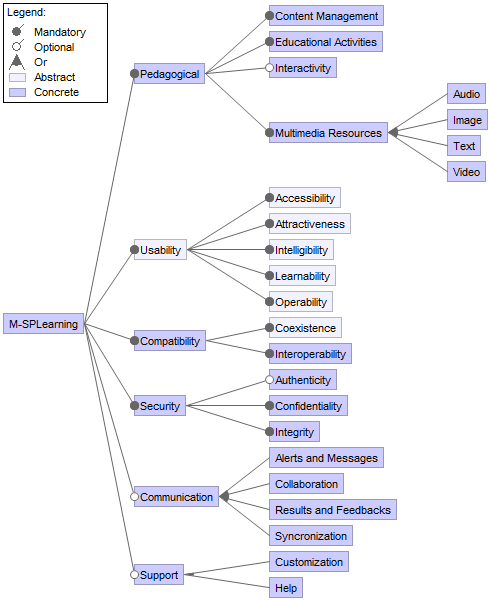
\includegraphics[width=0.91\textwidth]{MSPLFeatureModel.png}
\centering
\caption{\texttt{M-SPLear\allowbreak ning}: Feature Model.}
\label{fig:msplearning-fm}
\end{figure*}

Besides that, to standardize the variability management, SMarty was used in all the diagrams modeled for the \texttt{M-SPLear\allowbreak ning}: Architecture , Components Design and Production Plan. In this sense, one of its most representative assets is the architecture diagram (Figure \ref{fig:msplearning-architecture}). This diagram is the main artifact of the Architecture phase, because it presents the variabilities, commonalities and interactions between the SPL architectural components. Therefore, we have an overview of the product line and its domain modeling, essential information for the Design phase that details the responsibility of each component.

\begin{figure*}[!htbp]
\centering
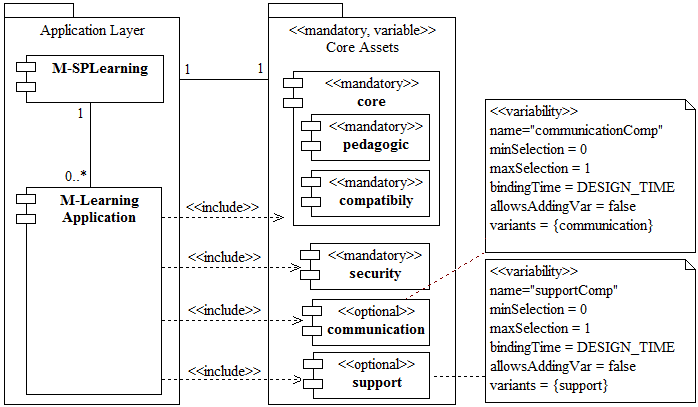
\includegraphics[width=0.92\textwidth]{MSPLArchitecture.png}
\centering
\caption{\texttt{M-SPLear\allowbreak ning}: Architecture (SMarty-based Component Diagram).}
\label{fig:msplearning-architecture}
\end{figure*}

Finally, with the support of these approaches and tools it was possible to instantiate our SPL, allowing an experimental evaluation of its products. In this sense, the Figure \ref{fig:msplearning-web} presents \texttt{M-SPLear\allowbreak ning}'s creation page, with the selection of variabilities for product generation. The following section details how the experiment was conducted to evaluate these products.

\begin{figure*}[!htbp]
\centering
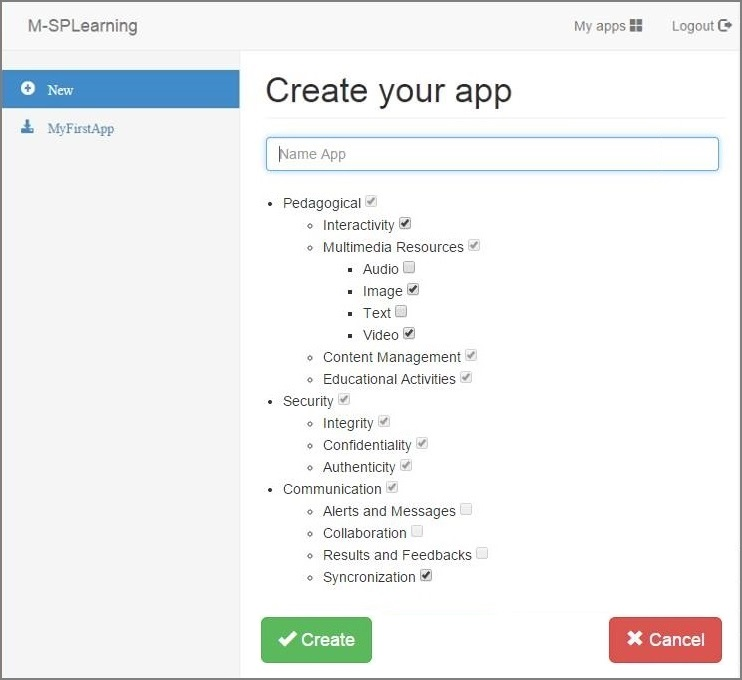
\includegraphics[width=0.75\textwidth]{MSPLWebGeneration.jpg}
\centering
\caption{\texttt{M-SPLear\allowbreak ning}: Product creation page.}
\label{fig:msplearning-web}
\end{figure*}


%TODO [OK] Sugestão: "Diluir" o  Background na Introducão para ter mais espaco para a M-SPLearning. Além disso, reduzir a secão de Trabalhos Relacionados (3 ou 4 parágrafos somente).


% 30/12/2015 06:22 %

\section{M-SPLear\allowbreak ning Experimental Evaluation}\label{section3}

%In this section, an experimental evaluation of M-SPLear\allowbreak ning regarding time-to-market and quality improvement in generating mobile learning applications is reported. M-SPLear\allowbreak ning was compared with a singular software development methodology. This study, we called as singular methodology the process of software development in which developers use only their own knowledge to develop mobile learning applications from scratch, without any reuse or support technique.  

In this section, an experimental evaluation of M-SPLear\allowbreak ning regarding time-to-market and quality improvement in generating mobile learning applications is reported. M-SPLear\allowbreak ning was compared with a singular software development methodology. It was adopted the term singular methodology as the process of software development in which developers use only their own knowledge to develop mobile learning applications from scratch, without any reuse or support technique.  

The guidelines proposed by Wohlin et al \cite{wohlin12} and the report template suggested by Jedlitschka and Pfahl \cite{jedlitschka07} were followed for the conduction of this controlled experiments.

\subsection{Motivation}\label{sub:motivation}


The choice for the adoption of new technologies or approaches used in the development process depends on several aspects of quality. Although many approaches have been developed, many issues about them must be solved for a suitable adoption in both industry and academic environments. Experimental evaluations may shed light on the identification of evidence from quality and benefits of an approach, justifying its choice. In some cases, the collected evidence may still support the correction of problems identified during the experimental evaluations and improvements in the proposals \cite{wohlin12,juristo10}.

Therefore, the experimental evaluation of M-SPLear\allowbreak ning is presented based on two relevant software development variables: time-to-market and number of faults. These variables can be directly influenced by the adopted development methodology and approaches that support the variabilities and commonalities management \cite{hubaux10,capilla13}. Additionally, in industry, quality and time-to-market, such as other variables, can define the success or unsuccess of the business to satisfactorily attend their clients \cite{hubaux10}. Thus, we select these variables to be experimentally compared in our study, considering the influence in the adoption of a concise variability management approach in the design phase of the M-SPLear\allowbreak ning.


\subsubsection{Research Objective}\label{sub:object}

The experiment aimed at \textbf{comparing} a singular software development (SSD) and the software product line (SPL) methodologies, \textbf{for the purpose of} identifying the most efficient, \textbf{with respect to} the time spent on the creation of software products and the number of faults found, from the point of view of software engineers \textbf{in the context of} practitioners from industry.


\subsection{Experimental Design}\label{sub:design}

This section describes the experimental design and procedures for support of future replications. In this sense, all the planning, configuration of environment, dynamics of execution and tests are in the experimental package, available on the project website\footnote{\url{http://falvojr-msc.github.io/msplearning}}.

\subsubsection{Goals}

Two research questions (R.Q.) based on the research objective were raised:

\begin{itemize}
\setlength\itemsep{0.8em}
\item \textbf{R.Q.1} Which methodology is more efficient regarding time-to-market -- singular software development (SSD) or SPL software product line (SPL)?
\item \textbf{R.Q.2} Which methodology presents more quality, in terms of number of faults, in the software product created -- SSD or SPL?
\end{itemize}

\subsubsection{Hypotheses}

Two sets of hypotheses were defined to be tested and each of them is related to its respective research questions (R.Q.1 and R.Q.2):

\vspace{1em}
\textbf{R.Q.1 hypotheses:} time-to-market

	\begin{itemize}
    \setlength\itemsep{0.8em}
	\item \textbf{Null Hypothesis ($H_{0}$)}: there is no significant difference of time-to-market between SSD and SPL. $(H_{0}$ : $\mu$(\textit{t(SSD)}) =  $\mu$(\textit{t(SPL)}));
	
	\item \textbf{Alternative Hypothesis ($H_{1}$)}: SSD has less time-to-market than SPL. 	($H_{1}$ : $\mu$(\textit{t(SSD)}) $<$ $\mu$(\textit{t(SPL)}));
		
	\item \textbf{Alternative Hypothesis ($H_{2}$)}: SSD has more time-to-market than SPL. 	($H_{2}$ :  $\mu$(\textit{t(SSD)}) $>$ $\mu$(\textit{t(SPL)})).		
	\end{itemize}	

\vspace{1em}
\textbf{R.Q.2 hypotheses:}
quality, in terms of number of faults
	\begin{itemize}
    \setlength\itemsep{0.8em}
	
	\item \textbf{Null Hypothesis ($H_{0}$)}: there is no significant difference between SSD and SPL with regard to quality regarding the number of faults in the software products created. 	($H_{0}$ : $\mu$(\textit{d(SSD)}) =  $\mu$(\textit{d(SPL)}));
	
	\item \textbf{Alternative Hypothesis ($H_{1}$)}: SSD has a larger number of faults than SPL. ($H_{1}$ : $\mu$(\textit{d(SSD)}) $>$ $\mu$(\textit{d(SPL)}));
		
	\item \textbf{Alternative Hypothesis ($H_{2}$)}: SSD has a smaller number of faults than SPL. ($H_{2}$ :  $\mu$(\textit{d(SSD)}) $<$ $\mu$(\textit{d(SPL)})).		
	
	\end{itemize}

\subsubsection{Variables}

Dependent variables are time ($t$) and faults ($f$), defined as follows:

\small

\begin{equation}\label{eq:1}
\mu{(t)}=(\Sigma xi)/n, i = 1..n
\end{equation}
\begin{equation}\label{eq:2}
\mu{(f)}=(\Sigma yi)/n, i = 1..n
\end{equation}
\normalsize 

where:

- \textit{t} is the implementation time (minutes);

- \textit{f} is the number of faults;

- \textit{xi} is the time of implementation of participant i;

- \textit{yi} is the number of faults detected in the implementation of participant i;

- \textit{n} is the total of participants in the experiment.

\normalsize


\vspace{5mm}


Independent variables are the development methodology, which is a factor with two treatments (SSD and SPL), and the software product configuration for mobile learning platform, which is a factor with two treatments, namely product 1 (P1) and product 2 (P2). Table \ref{tab:variables} shows the description of dependent and independent variables.

\begin{table}[ht]
\centering
\caption{Dependent and Independent Variables Description.}
\label{tab:variables}

\resizebox{1.0\textwidth}{!}{%
\begin{tabular}{|c|c|c|c|c|c|c|c|c|c|}
\hline
\textbf{\begin{tabular}[c]{@{}c@{}}Name of \\ the Variable\end{tabular}} & \textbf{\begin{tabular}[c]{@{}c@{}}Type of \\ the Variable\end{tabular}} & \textbf{Abbrev.} & \textbf{Class} & \textbf{Entity} & \textbf{\begin{tabular}[c]{@{}c@{}}Type of \\ Attribute\end{tabular}} & \textbf{\begin{tabular}[c]{@{}c@{}}Scale \\ Type\end{tabular}} & \textbf{Unit} & \textbf{Range} & \textbf{\begin{tabular}[c]{@{}c@{}}Counting \\ Rule\end{tabular}} \\ \hline
\begin{tabular}[c]{@{}c@{}}Development \\ methodology\end{tabular} & Independent & DM & Method & \begin{tabular}[c]{@{}c@{}}Software \\ development \\ methodology\end{tabular} & N/A & Nominal & N/A & SSD and SPL & N/A \\ \hline
\begin{tabular}[c]{@{}c@{}}Software \\ products\end{tabular} & Independent & P & Product & \begin{tabular}[c]{@{}c@{}c@{}}Mobile \\ software \\ product\end{tabular} & N/A & Nominal & N/A & P1 and P2 & N/A \\ \hline
\begin{tabular}[c]{@{}c@{}}Time of \\ implementation\end{tabular} & Dependent & t(3) & Product & \begin{tabular}[c]{@{}c@{}}Time to \\ market\end{tabular}  & \begin{tabular}[c]{@{}c@{}}Internal: time; \\ external: time \\ to market.\end{tabular} & Ordinal & Minutes & \begin{tabular}[c]{@{}c@{}}From 00:00:00 \\ to 03:00:00\end{tabular} & Eq. 1 \\ \hline
Faults & Dependent & f(4) & Product & \begin{tabular}[c]{@{}c@{}c@{}c@{}}Number of \\ faults \\ in each \\ software \\ product\end{tabular} & \begin{tabular}[c]{@{}c@{}}Internal: faults; \\ external: quality.\end{tabular} & Ordinal & Integer & Any integer & Eq. 2 \\ \hline
\end{tabular}%
}
\end{table}

Time-to-market is the time spent, in average, for the implementation of a software product with a specific group of variabilities of M-SPLear\allowbreak ning. With regard to the number of faults, the implemented products were tested using the concept of test cases \cite{craig02}. Thus, it was possible to quantify the mean of defects of products. Such metrics are relevant since they are directly related to time-to-market and quality of the m-learning applications. Additionally, they are relevant metrics for development industry\cite{JABANGWE201898}.

\subsubsection{Participants}

In our study, the participants were employees (volunteers) from a Brazilian software development industry. All of them had, at least, one year of experience with development background in Java, Microsoft .NET and/or PHP.

The small number of practitioners (18) led us to apply a non-random selection. The random capacity was applied at the assignment of the development methodology and software product by participant. 

It is important to highlight that, even with a small number of participants and a reduced statistical power, this experimental evaluation is important since it allows the collection of initial evidence about the compared methodologies. Besides, the sample can be increased in future replications \cite{falessi2017,host2000}.

Block classification was defined by two factors with two treatments, which were interspersed in four groups. The population was divided into four blocks by means of a draw. The balancing was applied in the tasks, which were assigned in equal numbers to a similar number of participants.

%The 18 participants were randomly separated into the following groups with a total of 9 participants each:

The 18 participants were randomly separated into groups of nine participants each:

\begin{itemize}
\item \textbf{First Group:} focused on SSD with P1 and SPL with P2;

\item \textbf{Second Group:} focused on SPL with P1 and SSD with P2;

\item \textbf{Third Group:} focused on SSD with P2 and SPL with P1; and

\item \textbf{Fourth Group:} focused on SPL with P2 and SSD with P1;
\end{itemize}

\subsubsection{Objects}

Among a total of 30 features and different configurations, two educational software products configurations for mobile learning platform (Android) were considered for the application of the SSD and SPL methodologies, which were: one for image (P1) and one for video resource (P2).

\subsubsection{Instrumentation}

The experiment was supported by the following set of instruments: (i) similar desktop computers with all necessary tools (Eclipse IDE and plugins); (ii) the consent term for the experimental study; (iii) a characterization questionnaire; (iv) use case, component and sequence UML diagrams; (v) interface messages; (vi) database model; (vii) a project base; (viii) similarities of the products; and (ix) experimental forms for SSD and SPL, randomly distributed and feedback questionnaire.

\subsubsection{Data Collection and Analysis Procedures}

The main assessment tools were the products developed based on two software specifications (P1 and P2) for mobile learning platform (Android), also available in the experimental package.

The M-SPLear\allowbreak ning was designed according to the catalog of requirements (Section \ref{section2}) and with 30 features, 16 mandatory and 14 optional for m-learning applications. A specific niche of features was used for the evaluation. The variabilities related to multimedia resources enabled the creation of up to 15 different products. P1 and P2 were specified and implemented by SSD and SPL methodologies. Figure \ref{fig:prod} shows the nuances between the products generated for the video feature.

%REMOVI (linha 157 - não achei a figura de referência):  (represented in Figure \ref{figureMSPLFeatureModel}) 

\begin{figure*}[!ht]
\centering
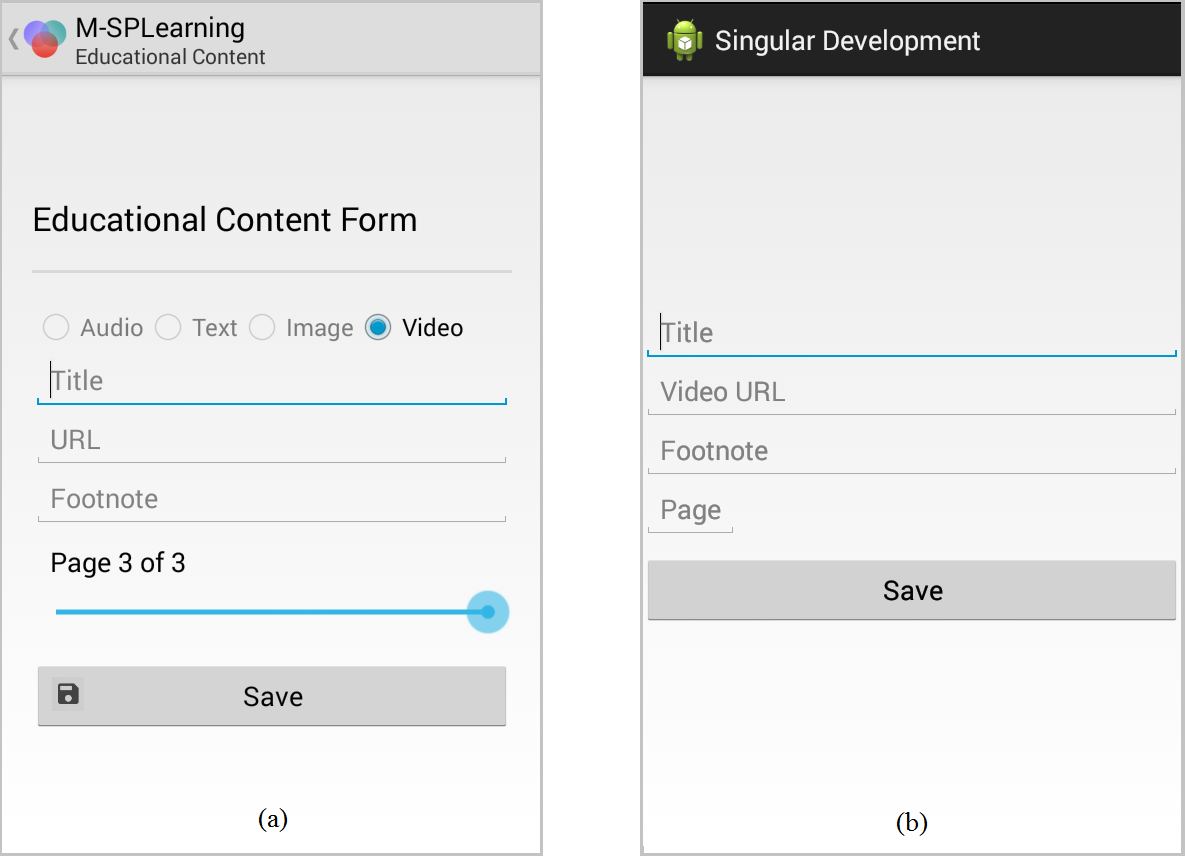
\includegraphics[width=0.69\textwidth]{MSPLGeneratedProducts.png}
\centering
\caption{Two Video Products (P1) Developed in the Experimental Execution with: (a) SPL and (b) SSD.}
\label{fig:prod}
\end{figure*}


To collect the data for the analysis of time-to-market, the initial and final time of implementation process for P1 and P2, was registered individually in the experimental form to be calculated in Equation \ref{eq:1}. On the other hand, for the analysis of quality, each of 15 developed products were tested and the number of faults was collect to compare the use of SPL and SSD methodologies by means of the Equation \ref{eq:2}.

\subsubsection{Validity Evaluation}

A pilot project was developed with two practitioners from industry, who evaluated the study instrumentation and established the duration of the training and execution sessions. The results and these participants were not considered in the final execution and data analysis of the experiment.

\subsection{Execution}\label{sub:execution}

This section presents how the experimental plan (design) was defined.

\subsubsection{Sample}

The sample was composed of a total of 21 practitioners, who participated in the training session. However, 18 participants contributed in the experimental execution, due the unavailability of three volunteers in the execution day.

\subsubsection{Preparation}

The participants underwent a three-day training session, in which were considered the essential concepts of Android development for SSD and SPL with the Eclipse IDE. The knowledge was evaluated through essays at the end of each training session. On the fourth day, the experiment was performed.

\subsubsection{Data Collection}

The steps adopted for data collection were:

\begin{enumerate}

\item The participants attended three days (four hours each day) of training sessions in an industrial environment;

\item The participants were divided into four groups by means of a draw;

\item The experimenter gave participants a set of documents containing UML diagrams, a dataset model and an interface message specification for each product, such as the material used in training session. Each participant was provided with a desktop computer with all requirements to develop a software product and an experimental form to register the spent time with the development process.
\item The participant read each given document;
\item The experimenter explained the documents;
\item The participant read and clarified possible doubts about the products specifications;
\item Each participant received and used two randomly drawn methodologies for the development of a requested m-learning product. For each application, participants registered the lasting of the application (start time, end and breaks). At the end of the two development tasks, for the two methodologies, they were asked to answer a feedback questionnaire and their opinion about the experimental execution and technologies used.
\end{enumerate}

\subsection{Analysis}\label{sub:analysis}

As the experiment session was finished, collected data was prepared (tabulation and descriptive statistics) in order to apply the statistical tests.

\subsubsection{Collected Data and Descriptive Statistics}

For each participant (``\texttt{Participant \#}'' column), we collected the following data: total time of implementation and total number of faults, identified by testing procedures, and the mean calculation. These results are shown in Table \ref{tab:resul1} and the results for each participant are plotted in box-plots of Figure \ref{fig:boxplot}. 

\begin{table}[ht]
\small
\centering
\caption{SSD and SPL Collected Data and Descriptive Statistics.}
\label{tab:resul1}
\resizebox{0.60\textwidth}{!}{%
\begin{tabular}{|c|c|c|c|c|}
\hline
\textbf{} & \multicolumn{2}{c|}{\textbf{SSD}} & \multicolumn{2}{c|}{\textbf{SPL}} \\ \hline
\textbf{Participant \#} & \textbf{Time (t)} & \textbf{Faults (f)} & \textbf{Time (t)} & \textbf{Faults (t)} \\ \hline
1 & 161 & 15 & 2 & 9 \\ \hline
2 & 90 & 8 & 1 & 0 \\ \hline
3 & 105 & 4 & 11 & 0 \\ \hline
4 & 104 & 1 & 3 & 0 \\ \hline
5 & 73 & 2 & 1 & 0 \\ \hline
6 & 99 & 9 & 3 & 0 \\ \hline
7 & 165 & 12 & 10 & 0 \\ \hline
8 & 95 & 1 & 3 & 0 \\ \hline
9 & 104 & 3 & 2 & 0 \\ \hline
10 & 102 & 0 & 4 & 0 \\ \hline
11 & 61 & 0 & 2 & 0 \\ \hline
12 & 82 & 4 & 8 & 0 \\ \hline
13 & 114 & 1 & 4 & 0 \\ \hline
14 & 103 & 6 & 14 & 0 \\ \hline
15 & 111 & 2 & 2 & 0 \\ \hline
16 & 176 & 9 & 4 & 0 \\ \hline
17 & 120 & 17 & 5 & 0 \\ \hline
18 & 175 & 34 & 2 & 9 \\ \hline
\textbf{Mean} & \textbf{113.33} & \textbf{7.11} & \textbf{4.50} & \textbf{1.00} \\ \hline
\textbf{Median} & \textbf{104} & \textbf{4} & \textbf{3} & \textbf{0} \\ \hline
\textbf{Std. Dev.} & \textbf{33.98} & \textbf{8.46} & \textbf{3.75} & \textbf{2.91} \\ \hline
\end{tabular}%
}
\end{table}

\begin{figure*}[!ht]
\centering
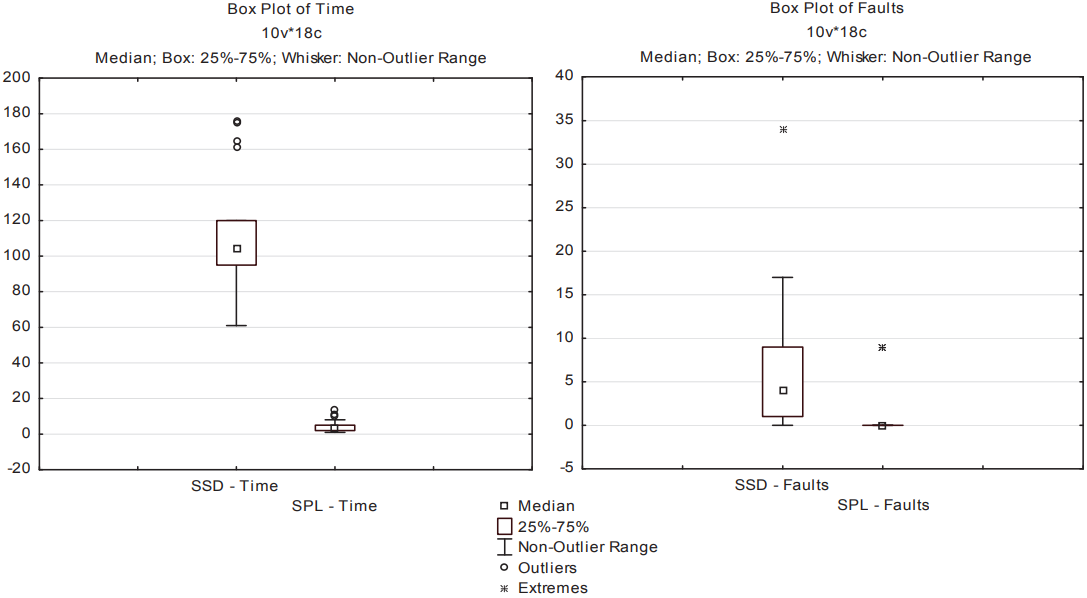
\includegraphics[width=1.0\textwidth]{MSPLBoxplotN.png}
\centering
\caption{Collected Data Box-Plot from SSD/SPL time-to-market and SSD/SPL faults.}
\label{fig:boxplot}
\end{figure*}

\subsubsection{Hypothesis Testing}

Based on the results obtained by the use of SSD and SPL to the development of two mobile learning products, we summarize, analyze and interpret the SSD and SPL collected data (Table \ref{tab:resul1} and Figure \ref{fig:boxplot}) by means of the Shapiro-Wilk normality test and the Mann-Whitney-Wilcoxon hypothesis test. Both tests validated the statistical power of the sample, allowing test the hypotheses.

\subsubsection{Efficiency in the Time of Implementation (R.Q.1)}

\begin{itemize}
\setlength\itemsep{0.8em}

\item \textbf{Collected Data Normality Tests:} Shapiro-Wilk \cite{shaphirowilk65} normality test was applied to SSD and SPL time and faults. The following results were obtained:\\

\textbf{\textit{SSD time (\textit{N}=18):}}

For mean value ($\mu$) of 113.33 and standard deviation value of ($\sigma$) 33.98, the time for the SSD was \textit{p} = 0.0274.

In the \textit{Shapiro-Wilk} test for a sample size \textit{(N)} 18 with 95\% of significance level ($\alpha$ = 0.05), \textit{p} = 0.0274 (0.0274 $<$ 0.05) and calculated value of \textit{W} = 0.8813 $<$ \textit{W} = 0.8970, the sample is considered non-normal.

\textbf{\textit{SPL time (\textit{N}=18):}}

For mean value ($\mu$) of 4.50 and standard deviation value of ($\sigma$) 3.75, the time for the SPL was \textit{p} = 0.0014.

For a sample size \textit{(N)} 18 with 95\% of significance level ($\alpha$ = 0.05), \textit{p} = 0.0014 (0.0014 $<$ 0.05) and calculated value of \textit{W} = 0.7978 $<$ \textit{W} = 0.8970, the sample is considered non-normal.

\item \textbf{Mann-Whitney-Wilcoxon for SSD and SPL time samples:} a rank with weights was assigned to each sample value. The weights were added and applied in Equation \ref{eq:MWW}:
\small
\begin{equation}
\label{eq:MWW}
U(DM) = N_1 * N_2 + \frac{N_1*(N_1+1)}{2} - \sum_{i=1}^{n} total_{2}
\end{equation}
\normalsize 

where:

- \textit{$U(DM)$} is the equation for each independent sample (DM);

- \textit{$N_1$} is the size of the sample for the X methodology;

- \textit{$N_2$} is the size of the sample for the compared methodology (Y);

- \textit{$total_{2}$} is the sum of the weights given for the compared methodology.
\normalsize 
\vspace{5mm}

The time values calculated by Equation \ref{eq:MWW} were 326.5 for SSD and 0.00 for SPL. Each weight matches the participants weights of development process time with SSD or SPL methodology. There is evidence that both values are different ($326.5>0$), which leads to the rejection of the null hypothesis ($H_0$) and acceptance of the alternative hypothesis ($H_{2}$).

Therefore, the answer to R.Q.1 is: SPL is more efficient than the SSD to implement software products for mobile platform taking into account the products P1 and P2 specification. The implementations of the base project and SPL were also considered in the experiment.

The participants received the base project of the two software products to be developed with SSD or SPL. It consisted of similarities of the products and was developed to reduce the experimental execution duration. It was implemented in 480 minutes (8 hours).

Based on the time spent in the development of each software product, it is possible to make some estimates related with the time efforts for both SSD and SPL methodologies evaluated. If considered the time required for the implementation of each base project adopting the SSD methodology, plus the total development time to each participants (480 minutes), the total time would be 10680 minutes or 178 hours ($total_{time}$((subje\allowbreak cts(18) x minutes(480)) + 2040 = 10680 minutes). 

On the other hand, taking into account the base project developing with SPL methodology, the time spent by the 18 participants was 81 minutes (1 hour and 21 minutes) and the total time would be 11361 minutes or 189 hours and 35 minutes ($total_{time}$((participants(18) x minutes(4.5)) + 10599 = 11361 minutes). 

Comparing the values, we notice that the SPL development spent 621 minutes (11 hours and 35 minutes) more than SSD. However, after the SPL implementation, this approach allows the evolution and insertion of new variabilities, assuring the faster generation of new products in addition to other advantages of the adoption of SPL approach.

\end{itemize}

\subsubsection{Number of faults of the created software products (R.Q.2)}

\begin{itemize}
\setlength\itemsep{0.8em}

\item \textbf{Collected Data Normality Tests:} 

\textbf{\textit{SSD faults (\textit{N}=18):}}

For a mean value ($\mu$) 7.11 and standard deviation value of ($\sigma$) 4, the fault for the SSD was \textit{p} = 0.0006 for the \textit{Shapiro-Wilk} normality test.

For a sample size \textit{(N)} 18 with 95\% significance level ($\alpha$ = 0.05), \textit{p} = 0.0006 (0.0006 $<$ 0.05) and value of \textit{W} = 0.7740 $<$ \textit{W} = 0.8970, the sample is considered non-normal.

\textbf{\textit{SPL faults (\textit{N}=18):}}

For a mean value ($\mu$) 1.00 and standard deviation value of ($\sigma$) 0, the fault for the SPL was \textit{p} = 0.00000007 for the \textit{Shapiro-Wilk} normality test.

For a sample size \textit{(N)} 18 with 95\% of significance level ($\alpha$ = 0.05), \textit{p} = 0.00000007 (0.00000007 $<$ 0.05) and value of \textit{W} = 0.3730 $<$ \textit{W} = 0.8970, the sample is considered non-normal.

\item \textbf{Mann-Whitney-Wilcoxon for SSD and SPL faults samples:} the number of faults calculated for SSD by Equation \ref{eq:MWW} was 282, whereas for SPL, it was 42.

Each weight matches participants development project faults with SSD or SPL methodology. There is evidence that both values are different ($282>42$), which leads to the rejection of the null hypothesis ($H_0$) and acceptance of the alternative hypothesis ($H_{1}$).

According to the result from the Mann-Whitney-Wilcoxon, the answer for R.Q.2 is obtained: it means that the SSD is prone to present more faults in the software products developed than the SPL. 

The faults found were identified based on test cases defined with a group of quality analysts from a software industry encompassing both SPL and SSD methodologies. These test cases considered the main functionalists of the expected software products. 

\item \textbf{Faults(SPL) x Faults(SS)}

Two type of faults were found for two participants that received the SPL methodology, one for each configuration (image (P1) and video (P2)). In both test cases it was expected the system to display a list of educational content, video or image types but they did not. 

For the SSD methodology, the faults were more serious. All the participants presented faults somehow. For the image (P1) and video (P2) software product, the faults where found in the same test cases: (i) the data was expected to be validated before be stored by the system in the data base of the process of creation of content; (ii) the system should present, but did not, a form with the educational content selected; and (iii) the  test case where the system should present a message of exclusion of content but, again, it was not presented. 

\end{itemize}

\subsection{Interpretation and Discussion}\label{sub:interpretation}

Data collected from the SSD and SPL application was analyzed and interpreted. The results are summarized in Table \ref{tab:resul_s}.

\begin{table}[ht]
\small	
\centering
\caption{SSD and SPL Normality and Statistical Tests Results.}
\label{tab:resul_s}
\resizebox{0.95\textwidth}{!}{%
\begin{tabular}{|c|c|c}
\hline
\textbf{Element} & \textbf{SSD} & \multicolumn{1}{c|}{\textbf{SPL}} \\ \hline
\textbf{Selection of Participants} & N(SSD) = 18 & \multicolumn{1}{c|}{N(SPL) = 18} \\ \hline
\multicolumn{3}{|c|}{\textbf{Time to Implementation}} \\ \hline
\textbf{Mean} & 113.33 & \multicolumn{1}{c|}{4.5} \\ \hline
\textbf{Shapiro-Wilk} & \begin{tabular}[c]{@{}c@{}}p = 0.0274 (p \textless 0.05)\\ Non-normal.\end{tabular} & \multicolumn{1}{c|}{\begin{tabular}[c]{@{}c@{}}p = 0.0014 (p \textless 0.05)\\ Non-normal.\end{tabular}} \\ \hline
\textbf{Mann-Whitney-Wilcoxon} & 326.5 & \multicolumn{1}{c|}{0} \\ \hline
\textbf{Result} & \multicolumn{2}{c|}{\begin{tabular}[c]{@{}c@{}c@{}}R.Q.1 H2: SPL has a smaller time-to-market \\ than SSD, based on evidenced statistical \\ difference of the time to implementation.\end{tabular}} \\ \hline
\multicolumn{3}{|c|}{\textbf{Number of Faults}} \\ \hline
\textbf{Mean} & 7.11 & \multicolumn{1}{c|}{1} \\ \hline
\textbf{Shapiro-Wilk} & \begin{tabular}[c]{@{}c@{}}p = 0.0006 (p \textless 0.05)\\ Non-normal.\end{tabular} & \multicolumn{1}{c|}{\begin{tabular}[c]{@{}c@{}}p = 0.00000007 (p \textless 0.05)\\ Non-normal.\end{tabular}} \\ \hline
\textbf{Mann-Whitney-Wilcoxon} & 282 & \multicolumn{1}{c|}{42} \\ \hline
\textbf{Result} & \multicolumn{2}{c|}{\begin{tabular}[c]{@{}c@{}}SPL has a smaller faults in the products \\ than SSD, based on evidenced statistical \\  difference of the number of faults.\end{tabular}} \\ \hline
\end{tabular}%l
}
\end{table}

In terms of time-to-market, the statistical difference showed by Mann-Whitney-Wilcoxon test provides evidence that SPL (i.e., M-SPLear\allowbreak ning) was more efficient than SSD in the development of P1 and P2 m-learning products; therefore, R.Q.1 has been answered.

Regarding the number of faults, the statistical difference presented by Mann-Whitney-Wilcoxon test provides evidence that SSD showed more faults than SPL in the development of P1 and P2 m-learning products); therefore, R.Q.2 has been answered.

According to the results of the Mann-Whitney-Wilcoxon test, both R.Q.1 and R.Q.2 null hypotheses can be rejected with a significance level of 95\% ($\alpha = 0.05$).

\subsubsection{Threats to Validity}\label{sec:threats}

This section addresses the actions taken to directly mitigate the threats of this experiment, according to the Conceptual Model of Anderlin Neto and Conte \cite{neto13} and Wohlin et al \cite{wohlin12}.

\vspace{1em}

\textbf{Internal Validity:}

\begin{itemize}
\setlength\itemsep{0.8em}
\item \textbf{Differences among participants:} as we selected participants with different experience levels, variations in their skills were reduced during the training sessions. The assessments conducted in the end of each day of training demonstrated the level of knowledge in the content used in the experimental execution and assured the reduction in variations in the participant skills. Even knowing that a more homogeneous sample reduces the participants representativeness, we decided to apply the training to reduce the heterogeneity of participants, that could threat the conclusion validity.

\item \textbf{Fatigue effects:} on average, the experiment lasted 180 minutes. Fatigue was not considered relevant since the participants could leave the room for a quick break. They were warned to not communicate during the breaks and, as a guarantee, a human observer supervised them. Periods of absence were registered and disregarded in the time analysed.

\item \textbf{Influence among participants:} the participants performed the experiment under the supervision of a human observer, then a possible influence of communication among them could be mitigated. As participants behave differently when being observed, training sessions allowed the adaptation the participants to the environment, reducing this threat.

\item \textbf{Training Sessions:} in the training sessions, explanations were given for every participant. This action was taken to avoid possible biases, and allow that every training member solve all his/her questions.
\end{itemize}

\vspace{1em}
\textbf{External Validity:}

\begin{itemize}
\setlength\itemsep{0.8em}

\item \textbf{Instrumentation:} m-learning products and other instruments were tested in the pilot project and were considered significant for the analysis of time-to-market and number of faults.

\item \textbf{Participants:} more experiments considering different metrics with industry practitioners must be conducted for the identification of other relevant factors related to the adoption of M-SPLear\allowbreak ning.

\end{itemize}

\vspace{1em}
\textbf{Construction Validity:} 

\begin{itemize}

\item \textbf{Independent Variables:} independent variables were tested in the pilot project to guarantee their validity.

\end{itemize}

\vspace{1em}
\textbf{Conclusion Validity:} 

\begin{itemize}

\item \textbf{Number of Participants:} since the number of participants was reduced, mainly by the availability of practitioners in the industry, the sample size must be increased in prospective replications of the experiment. Our results are considered indicators and are not conclusive, although the lack of experimental executions in an industrial environment, even with small samples, is important for the evaluation of the time-to-market and quality for both SSD and SPL approaches \cite{falessi2017,host2000}.

\end{itemize}


\section{Lessons Learned}\label{section4}

As the main lessons learned during the execution of the activities discussed herein, we highlight:

\begin{itemize}
\setlength\itemsep{1em}
\item \textbf{Domain Characteristics:} domain analysis can be considered one of the most important activity for the creation of an SPL. The evolution of the requirements catalog \cite{filho13} significantly contributed in terms of domain knowledge, supporting the adoption of the proactive model for the development of \texttt{M-SPLear\allowbreak ning}.
    
\item \textbf{Variability Management:} the adoption of SMarty helped in the identification of the variation points during the design of \texttt{M-SPLear\allowbreak ning}, ensuring more quality in the implemented components from the SPL. It also contributed to the better assimilation of the SPL concept. However, those involved must be trained accordingly, so SMarty can be used consistently.
    
\item \textbf{SPL Architecture:} SPL requires mechanisms to allow a transparent and easy manner to reflect all updates in the core assets in the architecture, and vice versa. That is, changes to the core assets require more efforts to maintain architectural integrity. Additional tools and analysis must be done to guarantee that all changes, or in the architecture or in the components, are reflecting all features and behaviors that the line has until that moment.
    
\item \textbf{SPL Development:} considering \texttt{M-SPLear\allowbreak ning}, the implementation of something generic and customizable is significantly different from a single-product-at-time approach. Therefore, developing features in an SPL requires a greater effort, which is justified by the subsequent gains of reuse \cite{clements02}.

On the other hand, the single-product development methodology hinders the maintenance of the products, without any rigorous development process defined. As all developers tend to program in their own way, giving support for each product developed, in most cases, can take more time and costs. If an SPL practice is adopted, being rigorously followed, time and cost to give support tend to decrease.
    
\item \textbf{Experimental Evaluation:} researches show that test executions in SPL are scarce and need to be evaluated and validated \cite{engstrom11}. Thus, the authors decided to apply the test cases in the products generated by the SPL, enabling an interesting comparison with an alternative methodology of development.

The experimental evaluation provided relevant results for the adoption of \texttt{M-SPLear\allowbreak ning}. The choice for active practitioners from the industry contributed to the reduction of the training session. However, experience and understanding of the concepts by the participants is always a difficult issue to be measured.

In addition, the use of testing techniques in the traditional development process and new ways to quickly test products from an SPL require more attention and research. One benefit in the adoption of SPL is about the quality improvement, since the products and their components are tested in several instances, leading to a quickly fix for the final client. Despite the use of the components in a large number of products and, consequently, for a higher number of target users for SPL, the way that the components and products were tested could be improved to be done in more aligned manner with the SPL specificities. Literature reflects more concern to test the SPL architecture in comparison to test the final components and products \cite{machado2014,net2011}.
\end{itemize}

\section{Related Work} \label{section5}

Our paper encompasses three main perspectives in industrial environments: (i) m-learning applications; (ii) SPL, with its benefits through variability management; and (iii) Experimental Software Engineering. Adopting SPL as methodology to develop m-learning applications allowed us to get positive evidence in a real industry environment about two measurable SPL benefits: quality of products and time-to-market, when experimentally compared with a singular software development process without a variability management approach to support the developers. Thus, our results come to complement the experiences related in other researches for these three perspectives.

In mobile applications development domain, Gamez et al \cite{gamez14} proposed a self-adaptation of mobile systems with dynamic SPL. The management of variabilities is achieved using the Common Variability Language (CVL). Marinho et al \cite{marinho10} proposed an architecture for nested SPL in the domain of mobile and context-aware applications. However, the authors did not specify how to improve the management of variabilities. Bezerra et al \cite{bezerra09} conducted a systematic review of SPL applied to mobile middlewares, but only six studies were significant for the review. According to the authors, the few results obtained highlight the need of more research in the area. 

These results led us to align the need of growing the number of m-learning applications, which still presents an incipient investigation in literature, using a reuse-based approach. In our case, we investigate the SPL methodology with the SMarty approach to manage the variabilities. Analysing the literature, as for m-learning development, there is also a lack of research in the use of SPL and variability management as a way to improve quality and time-to-market in industry. Chen and Babar \cite{chen11}, in a systematic literature review, concluded the status of evaluation of variability management approaches in SPL engineering was quite unsatisfactory. 

Jaring and Bosch \cite{jaring02} presented a case study in a Dutch-based company, Rohill Technologies BV -- a system development for, mainly, professional mobile communication infrastructures. They discussed and analyzed the need for handling variability in a more explicit manner, discussing the SPL and a method to represent and normalize variabilities. Some issues were highlighted, as the limited insight into the consequences of selecting a particular variability mechanism for variability identification; the need of a notation format to describe variability; and the fact that dependencies between variability and features are not made explicit to variability dependencies.

Hubaux et al \cite{hubaux10} combined variability representation and industrial case studies evaluations. They developed a Textual Variability Language (TVL) combining graphical and textual notations and performed an evaluation through a quantitative and qualitative analysis, considering four cases from different companies, sizes and domains. Positive benefits for TVL were identified, as the efficiency gained in terms of model comprehension, design and learning curve for the notation. Limitations were presented as well, such the difficulty in the adoption of the notation, since it can not be integrated in modeling tools. 

Eriksson et al \cite{eriksson09} also presented a language, but to manage requirements specifications for SPL. Using a qualitative evaluation -- document examination, participant observation and semi-structure interviews -- they compared the clone-an-own reuse with the proposed approach, which must be used together with a previously developed method to manage product line use cases models. Six variables were analyzed: adoption effort, expressiveness, scalability, ROI, risks and reuse infrastructure. The ROI variable presented negative results, whereas the others presented positive evidences for the proposed language. 

Still in the context of SPL evaluation in industry, but focusing on quality through software testing, Ardis et al \cite{ardis00} used the Family-Oriented Abstraction, Specification and Translation (FAST) approach as a development process for an SPL in a case study, covering all aspects of domain analysis with tests. According to the authors, test process in an SPL presents significant challenges. Thus, they presented, for each case study, three testing strategies suitable for general use in SPL testing: (i) testing common code thoroughly; (ii) exploiting common aspects of variable code; and (iii) using scenarios from the commonality analysis. 

Gacek et al \cite{gacek01} presented a case study regarding the adoption of SPL in a small company, called Market Maker. An holistic view of the challenges and changes in business was discussed, especially the automatization of tests in their developed components. Firstly, each single component was tested and, then, the entire system at runtime, using a special code inserted in each component. If an error occurred, the inserted test code identified automatically which component misbehave. The testing process was conducted only for components that were present in the instantiated product, i.e., components were not tested in their full flexibility, with respect to all possible instantiations in the family.

Batory et al \cite{batory02} defined a Product Line Architecture (PLA) with a Domain-Specific Language (DSL) to redesign an extensible command-and-control simulator for army fire support. In the case study, they collected preliminary results that PLA with DSL produce a more flexible way to implement the simulator and reduce the program complexity, if compared with the same simulator, with pure Java implementation. The complexity of the code was compared based on the number of methods, number of lines of code and tokens/symbols for both the adopted approach and the Java implementation.

%It is important to highlight that none of found related work allowed us to conduct a direct comparison with respect to our work.of results, since the focus of this evaluation are the time-to-market and quality (number of faults) applied in SPL and SSD methodologies. 


It is important to highlight that none of related work found in the literature allowed us to conduct a direct comparison with respect to our work.

The works of Hubaux et al \cite{hubaux10}, Eriksson et al \cite{eriksson09} and Ardis et al \cite{ardis00} proposed the specification of variabilities through language and graphical representations in industry case studies. In our research, the representation of variability was made using the  SMarty approach, which has already been evaluated in other experimental studies \cite{marcolino13,marcolino14a,marcolino14b,bera15,marcolinospl2017}.

Only two studies addressed some quality issues and tests, as our work. Ardis et al \cite{ardis00} defined a testing approach based on modeling test cases with an integer tuple. However, the proposed method was applied only in the context of SPL, not considering the SSD methodology. Gacek et al \cite{gacek01} adopted two-fold strategies in a case study to test the SPL products. Firstly, single components were tested by the developers themselves; secondly, the system was tested at runtime in the target environment using special test code inserted in each component. Similar to the Ardis et al \cite{ardis00} study, only the SPL methodology was considered, differing from our evaluation, which defined several test cases with a group of quality analysts from a software industry encompassing both SPL and SSD methodologies.


Finally, in spite of all related works having been  applied in industry, only few of them compared methodologies, such as SPL and singular development, highlighting which of these methodologies brings more quality and reduces time-to-market when supported by a variability management approach. Additionally, there still are several opportunities and open issues regarding the management of variabilities and experimental evaluation, particularly in the m-learning domain. This lack of researching in the area has motivated our work.

\section{Conclusions and Future Work}\label{section6}
 
This work presented M-SPLear\allowbreak ning -- an SPL that intends to support the systematic generation of m-learning applications on the Android platform. According to van der Linden et al \cite{vanderlinden07}, abstractions such as SPL allow the development process to be documented and reused systematically, contributing to the better comprehension of the target domain.

The main contribution of this work is related to the proposition of M-SPLearning and its experimental evaluation, which evidenced an improvement in the process of developing educational mobile applications through the use of SPL. In this scenario, the fault tolerance and time-to-market of such applications is essential to the end users. Therefore, there is a need of experimentally evaluating the products generated by the proposed SPL.

We experimentally evaluated the use of M-SPLear\allowbreak ning with respect to the singular software development. The obtained results were significant for the reuse approach, showing a reduction on time-to-market and a better quality in terms of number of faults when considering the software products developed with the support of variabilities. 

We also point out that the SMarty approach was crucial to the development of M-SPLear\allowbreak ning. The ease of import the SMarty Profile in a UML tool and the support provided by the SMarty Process in the application and recognition of variability have provided cost savings and better quality to the software products developed. Furthermore, with the experimental evaluations performed, improvements were applied in their elements, making SMarty a more complete and concise approach to be used. %These benefits justified its selection in our research.

%Como trabalhos futuros, pretende-se evoluir a M-SPLear\allowbreak ning com base nos insumos fornecidos a partir de sua avaliação empírica. Nesse sentido, ainda existe uma quantidade significativa de informações que podem induzir a novas linhas de pesquisa e avaliações experimentais.
As future work, we intend to evolve M-SPLear\allowbreak ning based on the inputs provided by the experimental evaluation performed. Actually, there is still a significant amount of information that can lead to new research lines and experimental evaluations. 
%Nesse sentido, novos experimentos estão sendo planejados em duas perspectivas: (i) replicação desta avaliação experimental, com o objetivo de aumentar o poder estatístico da amostra inicial; e (ii) projeto e execucão de novos experimentos, com o objetivo de avaliar a LPS e não seus respectivos produtos, como explorado neste trabalho. 
In this sense, other experiments have been planned in two perspectives: (i) replication of the experimental evaluation presented herein, in order to increase the statistical power of the initial sample; and (ii) design and execution of new experiments, aiming at evaluating SPL itself and not only its respective products, as explored in this work.

%Além disso, o modelo conceitual desenvolvido está em processo de avaliacão e modificação, considerando o domínio específico de ensino de programação. Com isso, estamos conduzindo mais estudos sobre esta adoção, possibilitando melhorias em nossa proposta e tornando-a mais adequada para adoção tanto na academia quanto na industria.

The conceptual model developed has also been evaluated and evolved, considering the specific domain of programming teaching. More studies on the adoption of M-SPLear\allowbreak ning in different contexts should enable improvements in our proposal, making it more suitable for the use in both academia and industry.

%Além disso, para que a M-SPLear\allowbreak ning possa ser avaliada em sua totalidade, todas as features elicitadas pelo catálogo de requisitos devem ser devidamente implementadas. Desta forma, um estudo empírico envolvendo a LPS propriamente dita pode ser conduzido, porque nosso experimento aferiu apenas os produtos da M-SPLear\allowbreak ning.
Moreover, for a complete evaluation of M-SPLear\allowbreak ning, all features elicited by the catalog requirements must be properly implemented. Therefore, an experimental study involving the SPL itself should be also conducted. %, since our experiment measured only M-SPLear\allowbreak ning products.

%Considerando o domínio explorado, a plataforma Android vem recebendo constantes contribuições em sua estratégia de desenvolvimento. Com isso, o aperfeiçoamento da M-SPLear\allowbreak ning deve sempre considerar a avaliação de novas ferramentas, fazendo com que a LPS evolua de acordo com as tendências do mercado.
%Considering the explored domain, the Android platform has received ongoing contributions to its development strategy. Thus, the improvement of M-SPLear\allowbreak ning must always consider the evaluation of new tools, causing the LPS evolve according to market trends.

%Para avaliação das evoluções da M-SPLear\allowbreak ning novos experimentos devem ser conduzidos, explorando vertentes relevantes para contexto educacional. Nesse sentido, avaliar os produtos gerados considerando variáveis como usabilidade e efetividade devem proporcionar resultados expressivos para este estudo. Além disso, as aplicações móveis resultantes podem ser aplicadas  em cenários reais de ensino e aprendizagem, com o objetivo de avaliar a M-SPLear\allowbreak ning aplicada ao seu domínio de usuários.
%evolutions of 

%To evaluate the M-SPLear\allowbreak ning new experiments should be conducted, exploring relevant  aspects to educational context. In this sense, evaluate the products considering variables such as usability and effectiveness should provide significant results for this study. In addition, the resulting mobile applications can be applied in real scenarios of teaching and learning, in order to evaluate the M-SPLear\allowbreak ning applied to its potential users.

%Outra perspectiva interessante está relacionada à investigação das outras estratégias de adoção propostas por. O modelo extrativo poderia ser aplicado a produtos externos a M-SPLear\allowbreak ning, com o objetivo de expandir suas features. Além disso, o modelo reativo poderia ser estudado como uma alternativa para evoluções futuras da LPS proposta.
Finally, we also intend to investigate the use of other adoption models \cite{krueger02}. For instance, the extractive model can be applied in similar products to those generated by M-SPLear\allowbreak ning, aiming at increasing the validity of similarities and variabilities specified. The reactive model can be investigated as an alternative to the evolution of the proposed SPL as well.

\bibliographystyle{apalike}
\bibliography{main}

\end{document}